\documentclass[dcc]{fcfmcourse}
\usepackage{teoria}
\usepackage[utf8x]{inputenc}
\usepackage{amsmath}
\usepackage{amsfonts,setspace}
\usepackage{listings}
\usepackage{color}
\usepackage{cancel}
\usepackage{epstopdf}
\usepackage{qtree}
\usepackage{fancyhdr}
\usepackage{tikz}
\usepackage{hyperref}
\usetikzlibrary{automata,positioning}
\pagestyle{fancy}
\cfoot{``Sometimes it is the people no one can imagine anything of who do the things no one can imagine." \\Alan Turing}
\definecolor{pblue}{rgb}{0.13,0.13,1}
\definecolor{pgreen}{rgb}{0,0.5,0}
\definecolor{porange}{rgb}{0.9,0.5,0}
\definecolor{pgrey}{rgb}{0.46,0.45,0.48}

\lstset{language=Java,
  showspaces=false,
  showtabs=false,
  breaklines=true,
  showstringspaces=false,
  breakatwhitespace=true,
  commentstyle=\color{porange},
  keywordstyle=\color{pblue},
  stringstyle=\color{pgreen},
  basicstyle=\ttfamily,
  moredelim=[il][\textcolor{pgrey}]{$ $},
  moredelim=[is][\textcolor{pgrey}]{\%\%}{\%\%}
}

\newenvironment{codebox} {\small \ttfamily \obeylines \begingroup \setstretch{-2.4}} {\endgroup}

\title{Auxiliar 8}
\course[CC3102]{Teoría de la Computación}
\professor{Gonzalo Navarro}
\assistant{Manuel Cáceres}
\assistant{Ian Letter}

% Si pasas el comando usedate a la clase, la fecha aparecerá bajo la lista de auxiliares.
% Puedes usar el formato de fecha por defecto de latex (y traducirla usando babel)
% o puedes escribir lo que quieras con el comando \date.
% \date{1 de Septiembre, 2015}

\begin{document}
\maketitle
\begin{center}
9 de Noviembre del 2016
\end{center}
\vspace{-1ex}
\begin{problems}
 \problem Construya una $MT$ que
 \begin{enumerate}[a)]
     \item Decida el lenguaje $\{w \in \{a,b\}^*\,\colon \#_{a}(w)=\#_{b}(w)\}$
     \item Calcule $f(n,m) = n\ mod\ m$
     \item Calcule $f(n,m) = \left \lfloor \frac{n}{m} \right\rfloor$
 \end{enumerate}
\problem Construya una $MT$ que calcule la función :
\begin{align*}
    f\colon \mathbb{N}\setminus \{0\} &\to  \mathbb{N}\setminus \{0\}\\
     n &\mapsto f(n) = n!
\end{align*}
\problem Considere una $MT$ donde la cinta es doblemente infinita (en ambos sentidos).
\begin{enumerate}[a)]
    \item Defínala formalmente junto con su operatoria.
    \item Muestre que este mecanismo es equivalente a una $MT$  normal.
\end{enumerate}
\end{problems}

\newpage
\begin{center}
{\huge \underline{Soluciones}}
\end{center}
\begin{problems}
\problem
\begin{enumerate}[a)]
    \item Esta $MT$ :
    \begin{center}
    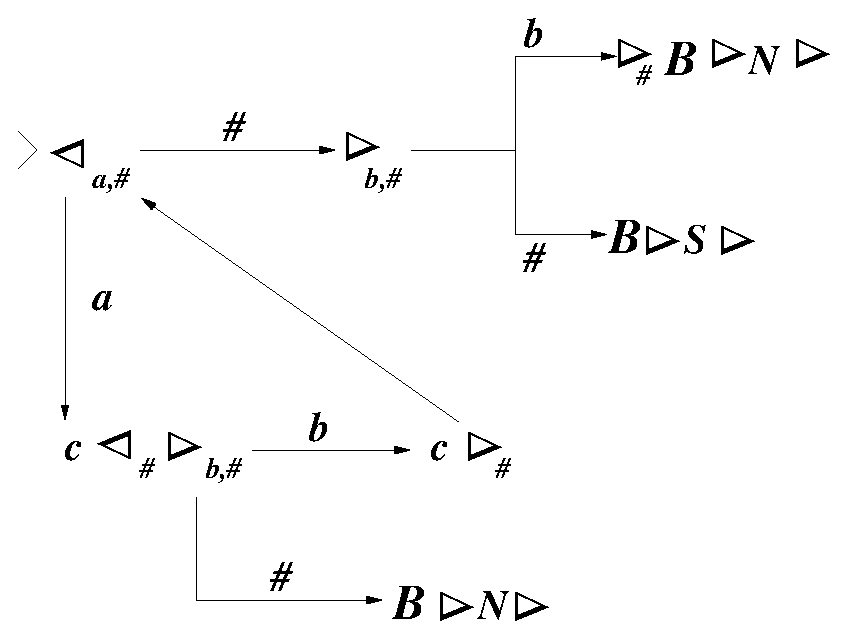
\includegraphics[scale=1]{P0a.eps}
    \end{center}
    \item Esta $MT$ :
    \begin{center}
    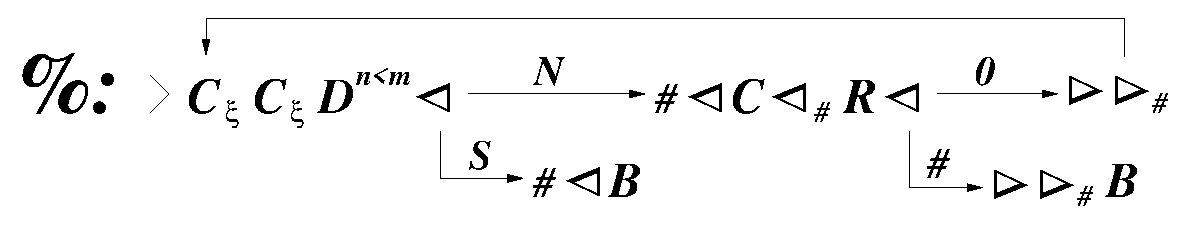
\includegraphics[scale=0.8]{P01b.eps}
    \end{center}
    \footnote{$C_{\xi}$ es la copiadora con salto ($\#x\#y\underline{\#}\rightarrow \#x\#y\#x\underline{\#}$).Agradecimientos a Cristóbal por fixear la máquina original.}
    \newpage
    Donde $D^{n<m}$ es la siguiente decididora:
    \begin{center}
    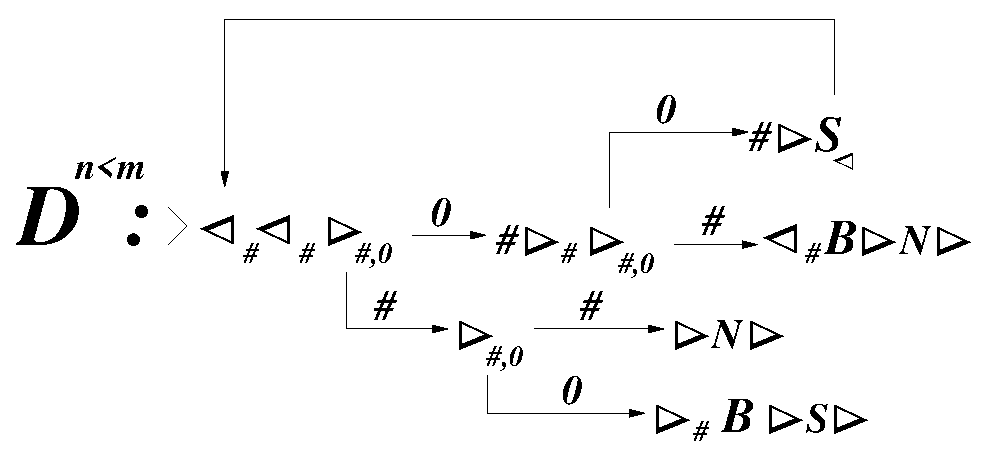
\includegraphics[scale=0.8]{P02b.eps}
    \end{center}
    \item 
    Recordamos que $n = m\left \lfloor \frac{n}{m} \right\rfloor + n\ mod\ m \Rightarrow \frac{n - n\ mod\ m}{m} = \left \lfloor \frac{n}{m} \right\rfloor \in \mathbb{Z}$, con esto en mente la $MT$ es la siguiente : % Hacer la division restando :D
    \begin{center}
    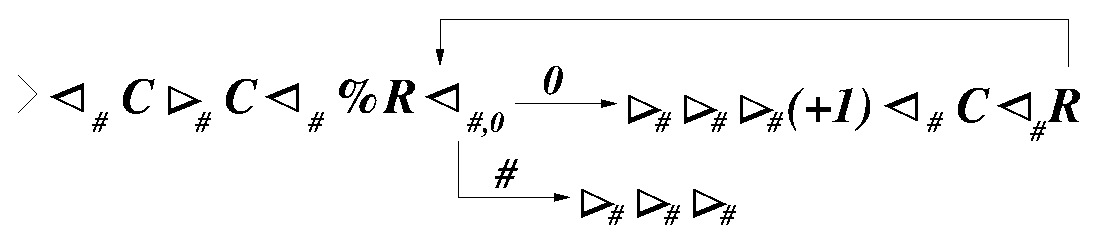
\includegraphics[scale=0.8]{P02c.eps}
    \end{center}
\end{enumerate}
\problem Usaremos dos cintas en las que mantendremos los invariantes:
\begin{align*}
    (1) &\quad \#0^{n^{\underline{k}}}\underline{\#}\\
    (2) &\quad \#0^{n-k}\underline{\#}
\end{align*}
La $MT$ es la siguiente:
\begin{center}
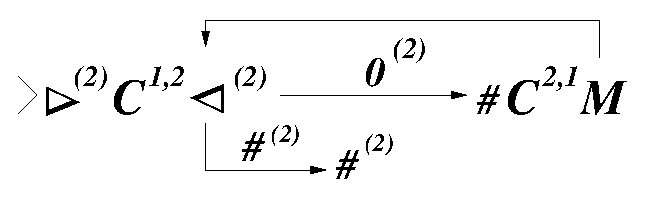
\includegraphics[scale=0.8]{P1.eps}
\end{center}
\newpage
Donde $C^{i,j}$ es la copiadora desde la cinta $i$ a la cinta $j$ y la $MT$ correspondiente es:
\begin{center}
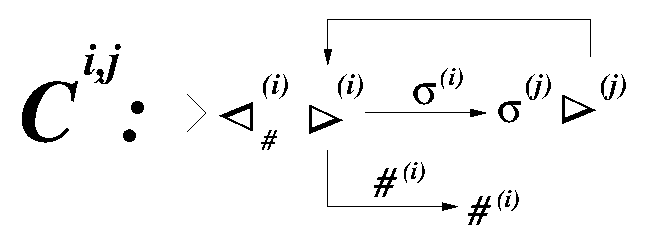
\includegraphics[scale=0.8]{P11.eps}
\end{center}
\problem 
\begin{enumerate}[a)]
    \item Al igual que en las máquinas normales, una $MT$ con cinta doblemente infinita es una tupla $M = (K,\Sigma,\delta,s)$. Con $K$ ($h\not\in K$) el conjunto de estados, $\Sigma$ el alfabeto de la cinta, $\delta\colon K \times \Sigma \to \left(K\cup \{h\}\right)\times \left(\Sigma \cup \{\triangleleft, \triangleright\}\right)$ (con $\triangleleft,\triangleright \not\in\Sigma$) la función de transición y $s$ el estado inicial.\\
    
    La principal diferencia con la $MT$ normal se da en la manera de computar de la máquina, lo que se refleja en las configuraciones y en la relación ``lleva en un paso''.\\
    
    Una configuración es un elemento del conjunto:
    \begin{align*}
        \mathcal{C}_{M} &= \left(K\cup \{h\}\right)\times\left(\Sigma^*\setminus\left(\{\#\} \circ \Sigma^*\right)\right)\times
        \Sigma \times \left( \Sigma^* \setminus \left( \Sigma^* \{\#\}\right)\right)
    \end{align*}
    La relación lleva en un paso entre configuraciones se define como :
    \begin{align*}
        (q,u\underline{a}v)\vdash_{M}(q',u'\underline{a}'v')\\
        \delta(q,a) = (q'b)
    \end{align*}
    \begin{itemize}
        \item Si $b\in\Sigma,\quad u'=u, v'=v, a'=a$
        \item Si $b=\triangleleft$
        \begin{itemize}
            \item Si $u \not = \epsilon,\quad u'a'=a$
            \begin{itemize}
                \item Si $av\not = \# \Rightarrow v'=av$
                \item Si no $\Rightarrow v' = \epsilon$
            \end{itemize}
            \item Si no $u'a' = \#, v'=av$
        \end{itemize}
        \item Si $b=\triangleright$
        \begin{itemize}
            \item Si $v \not = \epsilon,\quad a'v'=v$
            \begin{itemize}
                \item Si $ua\not = \# \Rightarrow u'=ua$
                \item Si no $\Rightarrow u' = \epsilon$
            \end{itemize}
            \item Si no $a'v' = \#, u'=ua$
        \end{itemize}
    \end{itemize}
    \newpage
    \item 
    \begin{itemize}
        \item Es claro que si tengo una $MT$ normal, puedo construir una $MT$ doblemente infinita que acepta el mismo lenguaje (las transiciones son las mismas, excepto que cuando la $MT$ normal se quiere mover a la izquierda en el inicio de la cinta, la doble pasa a un estado sumidero (esto se puede conseguir marcando en la cinta doble un punto como el ``inicio'' de la simple)).
        \item Por otro lado, si tengo una $MT$ doblemente infinita puedo construir una $MT$ de dos cintas (a partir de lo cual puedo construir una $MT$ normal, como se vió en cátedras) de modo que estas dos cintas simulan la cinta doblemente infinita, es decir, cuando la máquina doble quiere ir a la izquierda del inicio de la primera cinta pasa al inicio de la segunda cinta (para identificar esto marcamos los inicios de cada cinta) manteniendo las transiciones, con la salvedad de hacer ``al revés'' los movimientos del cabezal.
    \end{itemize}
\end{enumerate}
\end{problems}
\end{document}
